% Options for packages loaded elsewhere
\PassOptionsToPackage{unicode}{hyperref}
\PassOptionsToPackage{hyphens}{url}
\PassOptionsToPackage{dvipsnames,svgnames,x11names}{xcolor}
%
\documentclass[
  12pt,
]{article}

\usepackage{amsmath,amssymb}
\usepackage[]{crimson}
\usepackage{setspace}
\usepackage{iftex}
\ifPDFTeX
  \usepackage[T1]{fontenc}
  \usepackage[utf8]{inputenc}
  \usepackage{textcomp} % provide euro and other symbols
\else % if luatex or xetex
  \usepackage{unicode-math}
  \defaultfontfeatures{Scale=MatchLowercase}
  \defaultfontfeatures[\rmfamily]{Ligatures=TeX,Scale=1}
\fi
% Use upquote if available, for straight quotes in verbatim environments
\IfFileExists{upquote.sty}{\usepackage{upquote}}{}
\IfFileExists{microtype.sty}{% use microtype if available
  \usepackage[]{microtype}
  \UseMicrotypeSet[protrusion]{basicmath} % disable protrusion for tt fonts
}{}
\usepackage{xcolor}
\usepackage[margin = 1in]{geometry}
\setlength{\emergencystretch}{3em} % prevent overfull lines
\setcounter{secnumdepth}{5}
% Make \paragraph and \subparagraph free-standing
\ifx\paragraph\undefined\else
  \let\oldparagraph\paragraph
  \renewcommand{\paragraph}[1]{\oldparagraph{#1}\mbox{}}
\fi
\ifx\subparagraph\undefined\else
  \let\oldsubparagraph\subparagraph
  \renewcommand{\subparagraph}[1]{\oldsubparagraph{#1}\mbox{}}
\fi


\providecommand{\tightlist}{%
  \setlength{\itemsep}{0pt}\setlength{\parskip}{0pt}}\usepackage{longtable,booktabs,array}
\usepackage{calc} % for calculating minipage widths
% Correct order of tables after \paragraph or \subparagraph
\usepackage{etoolbox}
\makeatletter
\patchcmd\longtable{\par}{\if@noskipsec\mbox{}\fi\par}{}{}
\makeatother
% Allow footnotes in longtable head/foot
\IfFileExists{footnotehyper.sty}{\usepackage{footnotehyper}}{\usepackage{footnote}}
\makesavenoteenv{longtable}
\usepackage{graphicx}
\makeatletter
\def\maxwidth{\ifdim\Gin@nat@width>\linewidth\linewidth\else\Gin@nat@width\fi}
\def\maxheight{\ifdim\Gin@nat@height>\textheight\textheight\else\Gin@nat@height\fi}
\makeatother
% Scale images if necessary, so that they will not overflow the page
% margins by default, and it is still possible to overwrite the defaults
% using explicit options in \includegraphics[width, height, ...]{}
\setkeys{Gin}{width=\maxwidth,height=\maxheight,keepaspectratio}
% Set default figure placement to htbp
\makeatletter
\def\fps@figure{htbp}
\makeatother
\newlength{\cslhangindent}
\setlength{\cslhangindent}{1.5em}
\newlength{\csllabelwidth}
\setlength{\csllabelwidth}{3em}
\newlength{\cslentryspacingunit} % times entry-spacing
\setlength{\cslentryspacingunit}{\parskip}
\newenvironment{CSLReferences}[2] % #1 hanging-ident, #2 entry spacing
 {% don't indent paragraphs
  \setlength{\parindent}{0pt}
  % turn on hanging indent if param 1 is 1
  \ifodd #1
  \let\oldpar\par
  \def\par{\hangindent=\cslhangindent\oldpar}
  \fi
  % set entry spacing
  \setlength{\parskip}{#2\cslentryspacingunit}
 }%
 {}
\usepackage{calc}
\newcommand{\CSLBlock}[1]{#1\hfill\break}
\newcommand{\CSLLeftMargin}[1]{\parbox[t]{\csllabelwidth}{#1}}
\newcommand{\CSLRightInline}[1]{\parbox[t]{\linewidth - \csllabelwidth}{#1}\break}
\newcommand{\CSLIndent}[1]{\hspace{\cslhangindent}#1}

\usepackage{booktabs}
\usepackage{longtable}
\usepackage{array}
\usepackage{multirow}
\usepackage{wrapfig}
\usepackage{float}
\usepackage{colortbl}
\usepackage{pdflscape}
\usepackage{tabu}
\usepackage{threeparttable}
\usepackage{threeparttablex}
\usepackage[normalem]{ulem}
\usepackage{makecell}
\usepackage{xcolor}
\usepackage[scale = 0.8]{sourcecodepro}
\usepackage{etoolbox}
\makeatletter
\makeatother
\makeatletter
\makeatother
\makeatletter
\@ifpackageloaded{caption}{}{\usepackage{caption}}
\AtBeginDocument{%
\ifdefined\contentsname
  \renewcommand*\contentsname{Table of contents}
\else
  \newcommand\contentsname{Table of contents}
\fi
\ifdefined\listfigurename
  \renewcommand*\listfigurename{List of Figures}
\else
  \newcommand\listfigurename{List of Figures}
\fi
\ifdefined\listtablename
  \renewcommand*\listtablename{List of Tables}
\else
  \newcommand\listtablename{List of Tables}
\fi
\ifdefined\figurename
  \renewcommand*\figurename{Figure}
\else
  \newcommand\figurename{Figure}
\fi
\ifdefined\tablename
  \renewcommand*\tablename{Table}
\else
  \newcommand\tablename{Table}
\fi
}
\@ifpackageloaded{float}{}{\usepackage{float}}
\floatstyle{ruled}
\@ifundefined{c@chapter}{\newfloat{codelisting}{h}{lop}}{\newfloat{codelisting}{h}{lop}[chapter]}
\floatname{codelisting}{Listing}
\newcommand*\listoflistings{\listof{codelisting}{List of Listings}}
\makeatother
\makeatletter
\@ifpackageloaded{caption}{}{\usepackage{caption}}
\@ifpackageloaded{subcaption}{}{\usepackage{subcaption}}
\makeatother
\makeatletter
\@ifpackageloaded{tcolorbox}{}{\usepackage[many]{tcolorbox}}
\makeatother
\makeatletter
\@ifundefined{shadecolor}{\definecolor{shadecolor}{rgb}{.97, .97, .97}}
\makeatother
\makeatletter
\makeatother
\ifLuaTeX
  \usepackage{selnolig}  % disable illegal ligatures
\fi
\IfFileExists{bookmark.sty}{\usepackage{bookmark}}{\usepackage{hyperref}}
\IfFileExists{xurl.sty}{\usepackage{xurl}}{} % add URL line breaks if available
\urlstyle{same} % disable monospaced font for URLs
\hypersetup{
  pdftitle={Shades of Blue: Racial Imagery of Police and White Attitudes on Policing},
  pdfauthor={Chaoyue Wang},
  colorlinks=true,
  linkcolor={RoyalBlue4},
  filecolor={Maroon},
  citecolor={RoyalBlue4},
  urlcolor={Cyan4},
  pdfcreator={LaTeX via pandoc}}

\title{Shades of Blue: Racial Imagery of Police and White Attitudes on
Policing}
\author{Chaoyue Wang\footnote{Chaoyue R. Wang
  (\texttt{chyrwang@gmail.com}, \texttt{86-177-2387-5369}) is a senior
  student of Philosophy, Politics and Economics at Yuanpei College of
  Peking University, Beijing, China 100871.}}
\date{October 9, 2022}

\begin{document}
\maketitle

%----------------------------------------------
%   Abstract
%----------------------------------------------

\thispagestyle{empty}

\begin{abstract}  \onehalfspacing
\begin{normalsize}  \noindent 
Following the murder of George Floyd, whites and blacks again diverged
in their perceptions of and reactions to the reality of police violence
in the United States. Compared to people of color, white Americans are
more supportive of police agencies and more hesitant about reforming
policing behavior even in the wake of multiple recent unjustified
police-involved fatla shootings. While existing works look into
experiential and cultural differences between the two groups, this study
examines the role of whites' excessive representation in police
workforce that fosters a ``white imagery'' of the profession. Can this
racialized image of police officers activate in-group favoritism among
whites but push blacks away? Merging the 2020 Cooperative Election Study
with administrative sampling of local police departments, I find that
given whites' share of local population constant, a higher percentage of
white officers in local police department is associated with more
favorable feelings of police among whites, a greater black-white divide
in police attitudes, and makes the white residents more tolerant of
police at the presence of police violence.
\end{normalsize}
\end{abstract}

\begin{quote}
%\textbf{Keywords}: Keywords go here. \\
% \noindent \textbf{Note}: Note on replication data.
\end{quote}

%================Begin Manuscript==================
\newpage \clearpage \pagenumbering{arabic}\captionsetup{labelfont = bf, font = small}

\AtBeginEnvironment{tabular}{\small}

\AtBeginEnvironment{tablenotes}{\small}

\urlstyle{tt}

\ifdefined\Shaded\renewenvironment{Shaded}{\begin{tcolorbox}[enhanced, boxrule=0pt, breakable, sharp corners, interior hidden, borderline west={3pt}{0pt}{shadecolor}, frame hidden]}{\end{tcolorbox}}\fi

\setstretch{1.5}
\hypertarget{introduction}{%
\section{Introduction}\label{introduction}}

On May 25 of 2020, George Floyd, an unarmed 46-year-old African American
man, was choked to death in Minneapolis, Minnesota while a white local
police officer kneeled on his neck for over nine minutes. This blatant
instance of political brutality, along with multiple police-involved
homicides under intense public scrutiny, brings about a national debate
as to what the role of law enforcement should be and how policing
behavior should be regulated. Similar to many other debates in American
politics, a racial divide emerges in the public's response to police
violence. Compared to people of color, especially black and Hispanic
Americans, whites are in general more supportive of police officers and
less likely to view an unprovoked police shooting as abuse of police
power. In terms of reactions to heavily covered incidents of police
brutality, white people also is less approving of the Black Lives Matter
movement and less likely to appropriate police funding to other public
services.

Anecdotal insights have attributed this racial difference on policing
attitudes to white people's different living experiences with law
enforcement (\protect\hyperlink{ref-peffley2010}{Peffley and Hurwitz
2010}, \protect\hyperlink{ref-peffley2007}{2007}). White neighborhoods
are usually less surveilled by policing forces than their black or
Latino counterparts, and white people are also less likely to be stopped
or doubted than African and Hispanic Americans when displaying the same
amount of misconduct. Such racial discrimination against people of color
makes whites have in general fewer and more pleasant contact with
police, therefore rendering this population more favorable of the
performance of police officers.

In some experimental efforts to disentangle this racial divide, however,
it is found that even in the face of identical information on a
hypothetical situation of police-involved homicide, white subjects still
would draw a conclusion that is more supportive of police behavior than
black subjects (\protect\hyperlink{ref-jefferson2021}{Jefferson, Neuner,
and Pasek 2021}). Furthermore, this racial difference to the same
information is strongest among subjects that identify strongly with
their racial group, implying the existence of group dynamics underneath
this divide. But specifically, what dimension of one's racial identity
contributes to the fact that whites are anyway more supportive of police
officers at the presence of police violence? What part of group thinking
motivates white individuals to avoid addressing police officer's
objective responsibility?

This study approaches the puzzle of racial divide on policing attitudes
through a representation perspective. Police officer has been a
profession where white people are excessively represented both
historically and currently as to their share of local population. This
lasting over-representation of whites in police can forge a
stereotypical notion that sees police as ``whiter'' than the general
population. With this white imagery of police workforce in mind,
incidents of police violence may trigger white American's protective
feelings toward their racial in-group and thereby render them less
willing to update their beliefs on the reality of police misconduct. If
this is the case, we would expect weaker reception to political violence
information among white respondents that are served a police workforce
that is ``whiter'' than the population, and similarly, stronger
reception if their local police officers are better represented for
African and Hispanic Americans.

To test whether racial representation of local police moderates how
white Americans respond to police violence, this study draws three data
sources that respectively capture individual policing attitudes, racial
representation in local police, and local context of police violence.
The results find that even though white are not less willing to accept
the persuasion of police violence when whites are better represented in
local police, they do respond more critically to police violence if
local police workforce is more Hispanic or black than the local
population. In a word, racial imagination of police officers plays an
important role in how white people perceive police and understand police
violence.

\hypertarget{race-and-policing}{%
\section{Race and Policing}\label{race-and-policing}}

Following the murder of George Floyd, whites and blacks again diverged
in their perceptions of and reactions to the reality of police violence
in the United States. Compared to people of color, white Americans are
more supportive of police agencies and more hesitant about reforming
policing behavior even in the wake of multiple recent unjustified
police-involved fatla shootings. While existing works look into
experiential and cultural differences between the two groups, this study
examines the role of whites' excessive representation in police
workforce that fosters a ``white imagery'' of the profession. Can this
racialized image of police officers activate in-group favoritism among
whites but push blacks away? Merging the 2020 Cooperative Election Study
with administrative sampling of local police departments, I find that
given whites' share of local population constant, a higher percentage of
white officers in local police department is associated with more
favorable feelings of police among whites, a greater black-white divide
in police attitudes, and makes the white residents more tolerant of
police at the presence of police violence.

\hypertarget{empirical-strategy}{%
\section{Empirical Strategy}\label{empirical-strategy}}

\hypertarget{attitudes-on-policing}{%
\subsection{Attitudes on Policing}\label{attitudes-on-policing}}

To examine how racial imagery of local police shapes whites' perception
of policing and their attitudinal reactions to police violence, a data
source regarding the outcome variable needs to meet two requirements:
first, a diverse range of questions should be included that pertains to
the respondent's attitudes on the performance and the role of police.
Second, the place of the respondent's residence must be disclosed in the
dataset so that I can merge their policing attitudes to the local
context of police representation and police violence. The 2020
Cooperative Election Study (CES) meets both conditions. Unlike other
common public opinion surveys like American National Election Studies or
General Social Survey where a respondent's geographic information below
the state level is highly restricted for public access, CES of every
year discloses its respondent's place of residence as detailed as down
to the zip code level. Since the majority of police departments in the
United States are funded and operated on a municipality basis, the
precision of residence reported in CES allows us to match respondents
with the local context most immediate to their living experiences. On
the other hand, in the wake of the murder of George Floyd murder in the
June of 2020, the 2020 CES added to its questionnaire a battery of
questions regarding the respondent's perception of policing.

On a binary scale of yes or no, the 2020 CES asks the respondents
whether the presence of police makes them feel safe (``police felt as
safe''), whether they support increasing police funding at the expense
of sacrificing some budget for other public services (``increase
police''), and whether they are for decreasing police funding to better
support other public programs (``decrease police''). While the first
question tries to directly measure one's given perception of local
police, the latter two capture the respondent's attitudes on how police
should be maintained or regulated. To ease our interpretation of later
analyses, I linearly coerced the original responses so that for each
question, 1 indicates an affirmative response and 0 a negative one.

\hypertarget{racial-imagery-of-local-police}{%
\subsection{Racial Imagery of Local
Police}\label{racial-imagery-of-local-police}}

By the time when this study was conducted, there is no data source that
captures the universe of racial compositions of all police agencies in
the United States. To measure representation of different racial groups
in local police agencies, this study needs racial break of police
officers of a given police agency on the one hand, and racial structure
of the locality it serves on the other. For the first requirement, the
author chooses the 2016 Law Enforcement Management and Administrative
Statistics (LEMAS) that was collected by the Bureau of Justice
Statistics under the U.S. Department of Justice. Started in 1987, LEMAS
periodically collects data from more than 3000 state and local law
enforcement agencies, including all those that employ over 100 sworn
officers as well as a nationally representative sample of smaller police
agencies. Among the agency-level characteristics surveyed by LEMAS are
the demographic structure of their employees, the place they serve, and
their address in terms of zip code. Figure~\ref{fig-lemas-cover} shows
the county-level coverage of 2016 LEMAS sampling, where counties are
colored blue if at least one police department within its jurisdiction
is surveyed. Though apprarently having sampled more police departments
in more populated areas, the 2016 LEMAS in general has a geographically
comprehensive sample. Since most municipalities in the United States are
served by one police agency, it is reasonable to infer the police's
racial imagery of a place by looking at the racial compositions of its
local police employment. The author extracts from the 2016 LEMAS data
the total number of sworn officers in a police agency and the respective
numbers of white, Hispanic, and Black officers, and then calculates the
share of each racial group in the agency' employment.

\begin{figure}[tb]

{\centering 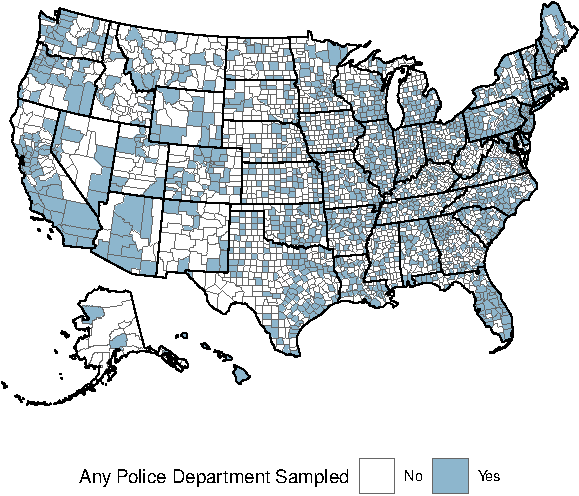
\includegraphics{quarto_files/figure-pdf/fig-lemas-cover-1.pdf}

}

\caption{\label{fig-lemas-cover}\textbf{Geographic Coverage of 2016
LEMAS at the County Level.} Counties are colored blue where at least one
police department within its jurisdiction is surveyed in 2016 LEMAS.}

\end{figure}

Given that the share of a racial group in police employment is a general
reflection of its percentage in local population, we can hardly
distinguish the effect of demographic structure from that of racial
composition of police officers if simply looking at the absolute value
of racial shares. A more precise approach would be to measure racial
representation in police by measuring the extent to which the presence
of a racial group exceeds or falls short of its presence in the local
population. This study hence measures racial representations in police
using the gap between the share of a racial group in police workforce
and in the total population of a place. On a positive-negative spectrum,
a large value of this difference for a racial group means that in this
place, a racial group is better represented in a police agency. For
example, if white Americans count for 70 percent of total population of
a city but over 90 percent of the city's police officers are white, then
black representation in police of the city would be 0.20, meaning an
excess of representation for whites in the police workforce and thereby
a ``whiter'' appearance of police officers.

Figure~\ref{fig-lemas-density} shows the distribution of racial
representations among the police departments surveyed in 2016 LEMAS. For
most police departments, whites are excessively represented in its
workforce, whose share notably exceeds their percentage in the overall
population. The median level of white representation is greater than 0
and its distribution is apparently right-skewed. For a considerable
number of departments, the level of excessive representation is beyond
0.2, creating a strongly whiter image of police officers.
Representations for African and Hispanic Americans, on the other hand,
present a opposite pattern. A dominant number of police departments
employ a smaller share of black or Hispanic police officers than their
presence in the population. The descriptive statistics found in 2016
LEMAS are consistent with the journalist and anecdotal evidence that
police employment is not representative of the population it serves,
forging a white imagery.

\begin{figure}[tb]

{\centering 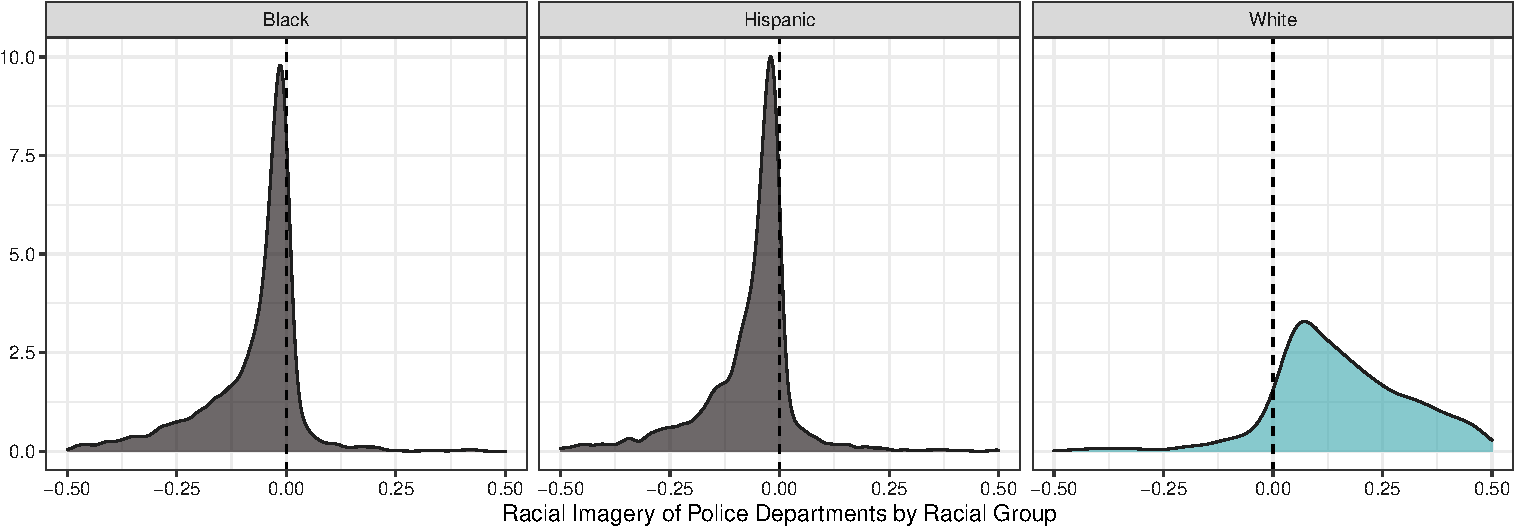
\includegraphics{quarto_files/figure-pdf/fig-lemas-density-1.pdf}

}

\caption{\label{fig-lemas-density}\textbf{Distribution of Racial
Presence among Police Departments Surveyed in LEMAS 2016.} Racial
imagery is measured by the difference between a racial group's share in
police officers and in local population. A positive value indicates that
the corresponding racial group is excessively represented in local
police departments, and a negative value the otherwise.}

\end{figure}

\hypertarget{local-police-violence}{%
\subsection{Local Police Violence}\label{local-police-violence}}

There have been no successful efforts by governmental agencies at either
local or federal level to systematically document police-involved
homicides. So existing literature addressing police violence has usually
turned to data voluntarily collected by advocacy groups, the most used
of which is that of Mapping Police Violence project. Drawing data points
from other reliable sources of police-involved shootings and collecting
its unique data through diverse channels including social media, local
newspaper accounts, and police reports, the Mapping Police Violence
project has by far the most detailed and accurate record of fatal
shootings by police since 2013.

Mapping Police Violence project reports where every police-involved
fatal shootings took place at zip code level along with what police
agency is responsible for the shooting. This allows this study to
connect CES respondents with their local context of police violence
using zip code and police agency information. To capture the occurrence
of police violence that are most immediate to a respondent's memory, I
focus on the those police-involved fatal shootings that took place in
2020 before September 29th, the date of the first surveying of 2020 CES.
The vast majority of the places where police violence happened saw only
one incident of such during the range of my observation, and outliers
with more than two police-involved homicides are rare, counting for less
than one percent of all observations. For this reason, I measure the
level of police violence on a binary basis, with 1 that there is at
least one case of police violence recorded in a place.

\hypertarget{results}{%
\section{Results}\label{results}}

\hypertarget{white-attitudes-on-policing}{%
\subsection{White Attitudes on
Policing}\label{white-attitudes-on-policing}}

Figure~\ref{fig-baseline} shows the estimates on the relationship
between racialized imagery of police workforce and whites' attitudes on
policing. Based on an individual regression among white respondents of
2020 CES, each point represents the estimated effect of the related
racial imagery (indicated by the horizontal axis) on one's policing
attitudes. As whites' presence in local police workforce increases
relative to its share in local population, whereby a ``whiter'' imagery
of police officers emerges, white Americans are more likely to claim
that police make them feel safe, and they are less willing to decrease
the funding for police to support other public services. No significant
effect of white imagery was found for the attitude on increasing police
funding, but the positive sign of the point estimate is consistent with
our expectation. In contrast, increased representation of African or
Hispanic Americans, which results in a police team that looks less like
white people, is associated with more negative feelings toward policing
among white Respondents. In either case, whites are less likely to
perceive police as safe or support an increase in police funding, and
are more likely to support decreasing police resources.

\begin{figure}[tb]

{\centering 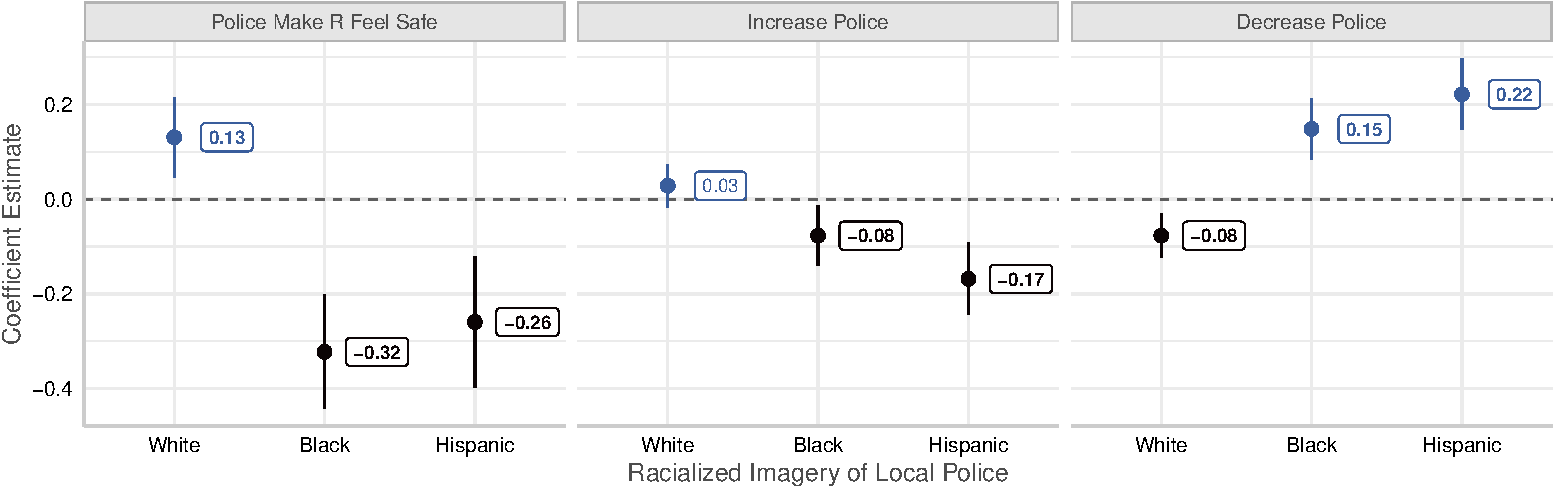
\includegraphics{quarto_files/figure-pdf/fig-baseline-1.pdf}

}

\caption{\label{fig-baseline}\textbf{The Estiamted Relationship between
Racial Imagery of Local Police and White Attitudes on Policing.} Each
point indicates the coefficient estimate of the realted racial imagery
on policing attitudes out of an invididual regression among white
respondents in 2020 CES. 95\% confidence intervals are shown by the
range. Outcome variable is indicated in the strip of each panel.
Positive estimates are colored blue and significant estimates are marked
in bold text. White percentage of local population is controlled.}

\end{figure}

Analyses in Table~\ref{tbl-divides} further looks into the extent to
which overall whiter imagery of police workforce contributes to the
current racial divide on policing attitudes. Here respondents of all
racial identities are included in the regressions. Taking the value of
the respondent's white identity, the term Racial Divide captures the
systemic difference between whites and people of color regarding their
attitudes on policing. Further, the interaction term between racial
divide and police's white imagery, when combined with the standalone
term of racial divide, estimates how racial imagery of police workforce
moderates the racial gap. Results indicate that regardless of the level
of police's white imagery, whites in general are more favorable of
police across the three attitudinal indicators. The racial gap on
feeling police as safe is exacerbated by a whiter imagery of police,
while the gaps on increasing or decreasing police funding are not.

\hypertarget{tbl-divides}{}
\begin{table}
\caption{\label{tbl-divides}Racial Imagery of Local Police Moderates Racial Divides on Policing
Attitudes }\tabularnewline

\centering
\begin{threeparttable}
\begin{tabular}[t]{lccc}
\toprule
  & Police Felt as Safe & Increase Police & Decrease Police\\
\midrule
Racial Divide & 0.443*** & 0.048** & -0.072***\\
 & (0.033) & (0.016) & (0.016)\\
White Imagery of Police & -0.335*** & 0.003 & 0.018\\
 & (0.097) & (0.048) & (0.048)\\
Racial Divide × White Imagery & 0.363** & 0.019 & -0.039\\
 & (0.111) & (0.057) & (0.055)\\
\midrule
Observations & 39551 & 39597 & 39589\\
R squared & 0.076 & 0.002 & 0.007\\
\bottomrule
\end{tabular}
\begin{tablenotes}
\item Note: All respondents in 2020 CES. The term Racial Divide takes the value of the respondents white identity, 1 if white and 0 if not white, thereby capturing the difference of whites on policing attitudes as compared to people of color. Robust standard errors in parentheses. + p $<$ 0.1, * p $<$ 0.05, ** p $<$ 0.01, *** p $<$ 0.001.
\end{tablenotes}
\end{threeparttable}
\end{table}

But when we are concerned about not the continuous variation of racial
gap but whether there is a gap at all, a different landscape shows up.
Building upon the OLS results in Table~\ref{tbl-divides},
Figure~\ref{fig-divides} presents whether the racial gap on policing
existed as a function of white imagery of police. Ranges where the
effect of white identity is not significantly from 0 at the level of
0.95 are colored red and indicated by blue reference lines. As the white
imagery of local police decreases, we see that the racial gap in feeling
police as safe notably declines and eventually diminished when the
police workforce are least white. For the attitudes on increasing or
decreasing police funding, even though less variation across levels of
racial imagery is found, it is still clear that when whites become
insufficiently represented in police workforce, the racial gap slightly
declines and are eventually not significant. This means that in places
where police officers appear less white, whites and people of color are
generally not so divided or not divided at all with regard to their
perceptions and visions for policing.

\begin{figure}[tb]

{\centering 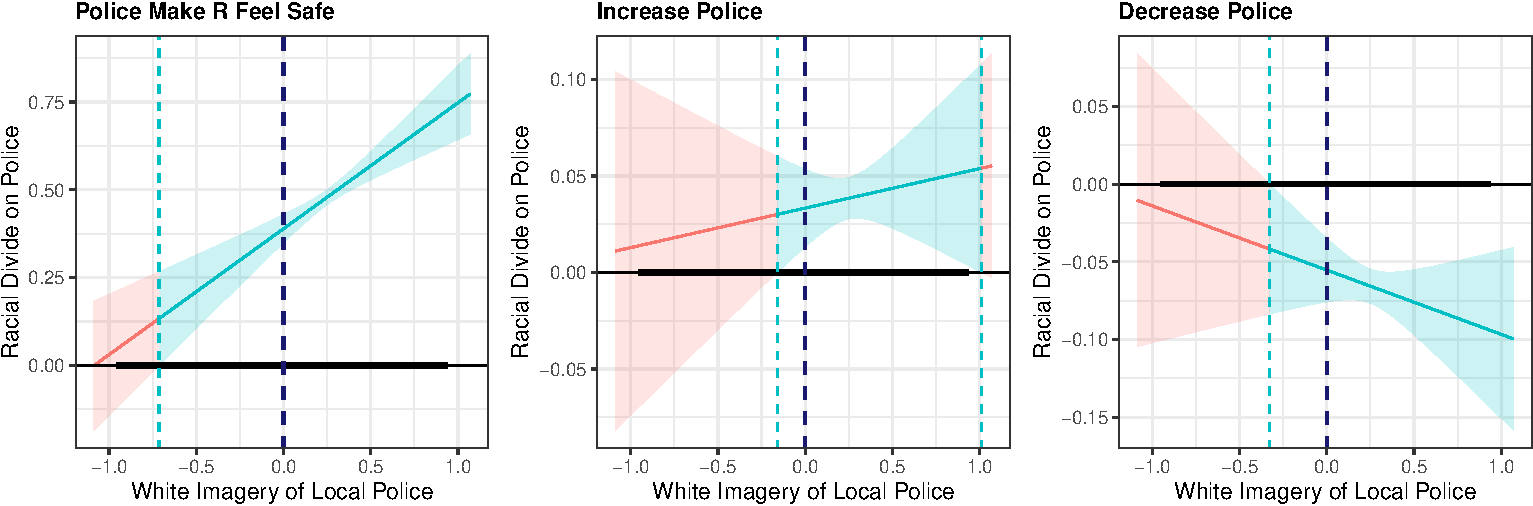
\includegraphics{quarto_files/figure-pdf/fig-divides-1.pdf}

}

\caption{\label{fig-divides}\textbf{Racial Imagery of Local Police
Moderates Racial Divide regarding Attitudes on Policing.} Each plot
shows the racial divide on the outcoem policing attitude as the white
imagery of local police increases. Ranges of racial imagery where racial
divide diminishes are colored red and indicated by blue reference
lines.}

\end{figure}

The results from the analyses above builds up our confidence that racial
imagery of police workforce, specifically the racial compositions of
local police officers relative to the racial structure of local
population, is a shaping force on white people's attitudes on policing.
As the police team gets ``whiter'', whites are more favorable of the
role of police. Racial imagery of police also affects the racial gap on
policing attitudes, places with higher representation of whites in
police employment seeing a larger racial divide. Based on these finding,
in the next part we turn to how racial imagery of police moderates white
people's attitudinal responses in the after of police-involved fatal
shootings.

\hypertarget{white-reaction-to-police-violence}{%
\subsection{White Reaction to Police
Violence}\label{white-reaction-to-police-violence}}

Table~\ref{tbl-reaction} shows the moderating effect of racial imagery
of police on white people's reaction to local police violence. Quite
intuitively, the occurrence of police violence during has a negative
impact on white's perception of policing, making them less likely to
feel police as safe or support increasing police funding, and more
likely to considering cutting police funding in support of other public
services. But this attitudinal reaction of whites to police violence is
strongly moderated by the racial imagery of local police, with the
interaction term significantly going against the sign of the main term.
As local police possess a more white imagery, the happening of police
violence is less effective in pushing whites toward more negative views
on policing.

Plotting linear predicted values of policing attitudes based on results
in Table~\ref{tbl-reaction}, Figure~\ref{fig-reaction-mod} communicates
this moderating effect of racial imagery of police in more
straightforward way. At the each given level of white imagery of police,
the distance between the black point and the green point indicates the
impact of police violence occurrence on white people's policing
attitudes. We can see that across the three attitudinal outcome
variables, the happening of police violence results in the greatest
shift of white attitudes when whites are insufficiently represented in
police workforce (-0.1). As the representation level of whites in police
rise to 0.2, thereby producing a ``whiter'' imagery of police, the
attitudinal shift is weakened but still existing. When whites are
overwhelmingly over-represented in police, however, almost no difference
is observed between those facing local police violence and those who are
not, indicating a diminishing of the persuasion effect of police
violence occurrence. Overall, greater white presence in police workforce
renders whites of a place more resistant to updating their attitudes on
policing even in the face of the occurrence of police-involved fatal
shootings.

\hypertarget{tbl-reaction}{}
\begin{table}
\caption{\label{tbl-reaction}Racial Imagery of Local Police Moderates Racial Reaction to Police
Violence. }\tabularnewline

\centering
\begin{threeparttable}
\begin{tabular}[t]{lccc}
\toprule
  & Police Felt as Safe & Increase Police & Decrease Police\\
\midrule
Any Police Violence in 2020 & -0.140*** & -0.057*** & 0.074***\\
 & (0.023) & (0.013) & (0.013)\\
White Imagery of Police & 0.018 & -0.009 & -0.014\\
 & (0.054) & (0.029) & (0.029)\\
Police Violence × White Imagery & 0.260** & 0.078+ & -0.142**\\
 & (0.083) & (0.045) & (0.045)\\
\midrule
Observations & 26016 & 26039 & 26036\\
R squared & 0.004 & 0.002 & 0.003\\
\bottomrule
\end{tabular}
\begin{tablenotes}
\item Note: Non-Hispanic white respondents only, 2020 CES. Robust standard errors in parentheses. + p $<$ 0.1, * p $<$ 0.05, ** p $<$ 0.01, *** p $<$ 0.001
\end{tablenotes}
\end{threeparttable}
\end{table}

\begin{figure}[tb]

{\centering 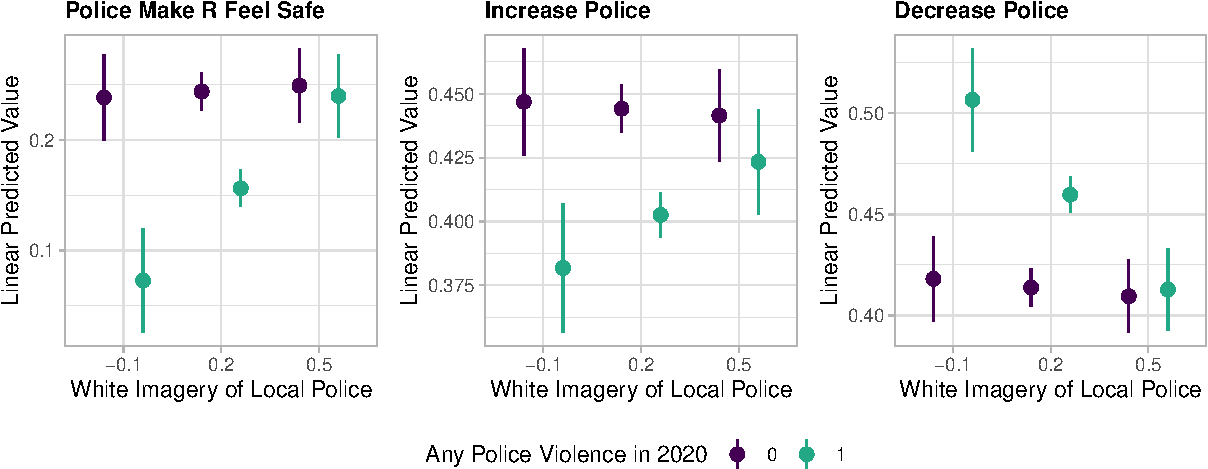
\includegraphics{quarto_files/figure-pdf/fig-reaction-mod-1.pdf}

}

\caption{\label{fig-reaction-mod}\textbf{Racial Imagery of Local Police
Moderates Whites' Attitudinal Response to Police Violence.} Based on the
previous OLS analyses with interaction terms, points here represent
linear predicted values of policing attitudes at different levels of
police violence occurrence and racial imagery of local police. At the
each level of racial imagery, whether there police violence happended in
2020 is indicated by the black-green scheme.}

\end{figure}

\hypertarget{examining-the-racial-component}{%
\subsection{Examining the Racial
Component}\label{examining-the-racial-component}}

So far we have observed that as white presence in police workforce
increases, whites will present more favorable views toward policing,
widen their gap on policing attitudes compared to people of color, and
are more resistant to updating their attitudes in the aftermath of
police violence. But how much of this association be attributed to the
racial in-group favoritism fostered among by whites by a ``whiter''
imagery of police officers? Since 2020 CES does not include in its
questionnaire detailed, in-depth questions regarding one's racial
attitudes or racial consciousness, this study is unable to directly
validate the mechanism. But if it can be shown that the effect of
police's white imagery is strongest in situations where racial dynamics
are emphasized or policing itself is scrutinized racially, we can have
some confidence that some sort of racial consideration is what drives
whites to favor police at the presence of a more white police workforce.

Based upon analyses into how racial imagery of police moderates white's
attitudinal response to police violence, this study further separates
the respondents into three categories based on whether police violence
took place in their locality during 2020, and the racial groups impacted
by such police violence. The first group of respondents is those who do
not have police-involved fatal shootings in their place of residence
(``No PV''). The second group live in places where at least one case of
police violence happened, but at least one victim impacted by such
violence is white (``PV Whites''). Similar to the second group, the
third group also sees at least one incident of police violence during
2020, but all racially identifiable victims are people of color (``PV
POC''). Police violence are more likely to activate concerns of racial
justice when predominantly involving people of color. Therefore, though
both affected by police violence, the third group differs from the
second in the sense that racial consciousness may be more prominent to
one's thinking in a more racialized context of police violence. If there
is a racial component in the relationship between police's racial
imagery and white attitudes on policing, we would expect that the
moderation effect of racialized police imagery may be stronger among the
third group than the second.

Table~\ref{tbl-racial.component} shows the results of our analyses.
Whites' attitudes on policing become less favorable both when police
violence impacts purely people of color and when such violence involves
at least one white victim. But the moderation effect of white imagery of
police is strongest or only present in the case of highly racialized
police violence. For the outcome variable of the respondent feeling
police as safe, whites are less likely to negatively update their views
in the face of police violence if police workforce sees better
representation for whites. This countering effect of racial imagery is
stronger when police violence purely impacts people of color than when
it involves one white victim. For the attitudes on increasing or
decreasing police, however, the moderation effect of police's white
imagery vanishes if at least one white victim is involved in police
violence.

\hypertarget{tbl-racial.component}{}
\begin{table}
\caption{\label{tbl-racial.component}Racial Imagery of Local Police Moderates Whites' Attitudinal Response to
Police Violence. }\tabularnewline

\centering
\begin{threeparttable}
\begin{tabular}[t]{lccc}
\toprule
  & Police Felt as Safe & Increase Police & Decrease Police\\
\midrule
PV Whites & -0.129*** & -0.039* & 0.056***\\
 & (0.030) & (0.016) & (0.016)\\
PV POC & -0.152*** & -0.077*** & 0.093***\\
 & (0.029) & (0.016) & (0.016)\\
White Imagery of Police & 0.015 & -0.013 & -0.010\\
 & (0.055) & (0.029) & (0.029)\\
White Imagery × PV Whites & 0.196+ & -0.003 & -0.075\\
 & (0.107) & (0.057) & (0.057)\\
White Imagery × PV POC & 0.327** & 0.162** & -0.210***\\
 & (0.106) & (0.058) & (0.058)\\
\midrule
Observations & 26016 & 26039 & 26036\\
R squared & 0.004 & 0.002 & 0.003\\
\bottomrule
\end{tabular}
\begin{tablenotes}
\item Note: Non-Hispanic white respondents only, 2020 CES. PV Whites means at least one victim of local police violence during 2020 is white. PV POC means that all victims of local police violence during 2020 are people of color. Robust standard errors in parentheses. + p $<$ 0.1, * p $<$ 0.05, ** p $<$ 0.01, *** p $<$ 0.001
\end{tablenotes}
\end{threeparttable}
\end{table}

Figure~\ref{fig-racial-component} illustrates more clearly the
heterogeneity of moderation effect of racial imagery contingent upon the
racialization of police violence. Plotting linear predicted values of
policing attitudes based on results in Table~\ref{tbl-racial.component},
Figure~\ref{fig-racial-component} shows at given levels of white imagery
of police, how white attitudes change in response to different types of
police violence, which are indicated by a group of points with different
colors. When white imagery of police violence is low (0.0), we see that
police violence has great persuasion effect regardless of their victims,
resulting in a notable distance from the baseline points of no police
violence. As white imagery of police violence rise to 0.5, thereby
fostering the perception of police officers as predominantly white, we
see that the attitudinal shit caused by police violence is smaller. When
police violence involves at least one white victim, the shift, though
small, is still observable in terms of point estimates. But when police
violence purely victimizes people of color, we see that the occurrence
of such violence not only fails to shift policing attitudes negatively,
but even pushes the point estimates toward more favorable direction. To
summarize, the fact that the moderation effect of racialized police
imagery is contingent upon the racialization of police violence lends
confidence to our hypothesis that a racial component lies underneath the
association between racial imagery of police and white attitudes on
policing.

\begin{figure}[tb]

{\centering 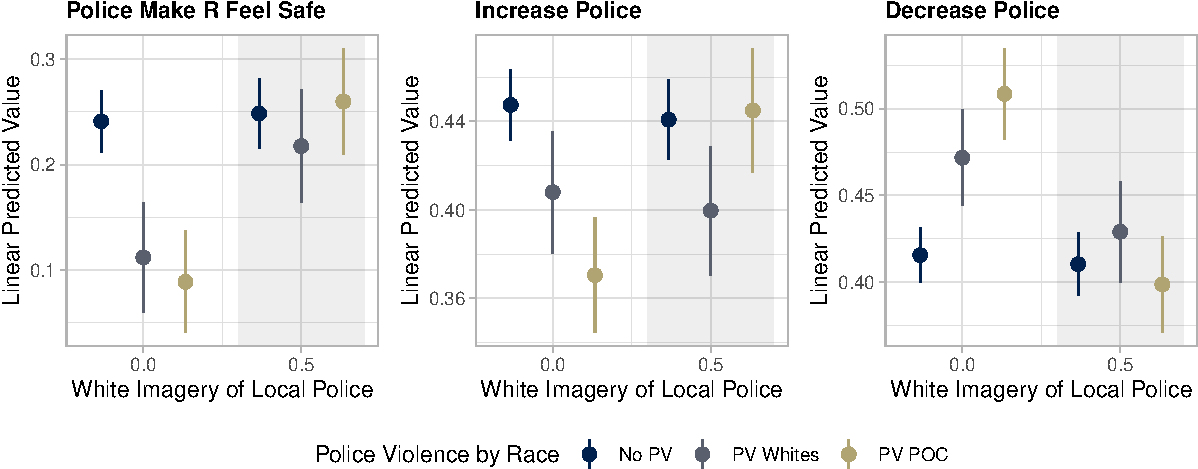
\includegraphics{quarto_files/figure-pdf/fig-racial-component-1.pdf}

}

\caption{\label{fig-racial-component}\textbf{Moderating Effect of Racial
Imagery Depends upon Racial Groups Victimized by Police Violence.} Based
on the previous OLS analyses with interaction terms, points here
represent linear predicted values of policing attitudes at different
types of police violence victimization and levels of racial imagery of
local police. At the each level of racial imagery, the racial groups
impacted by local police violence in 2020 are indicated by the
black-to-yellow scheme.}

\end{figure}

\hypertarget{conclusion}{%
\section{Conclusion}\label{conclusion}}

Looking into how racial imagery of local police moderates the way white
respondents respond to police violence, this study offers an
identity-oriented insight for disentangling the racial divide in
policing attitudes. The occurrence of police violence persuades white
residents of a locality to take up more critical views toward law
enforcement, but this persuasion effect is far stronger if the local
police confronting them is less white, that is, if the local police is
better represented for black and Hispanic Americans and thereby breaks
the anecdotal myth that police is largely a white profession. Further
more, the frequency of police violence can help narrow down the division
between whites and people of color on policing attitudes. This closing
effect on racial gap is also conditioned by racial representation of
local police, and will be stronger with a police department that has
more representation for black and Hispanic Americans. In conclusion,
white Americans' persistence on policing attitudes is at least partly
due to their over-representation in police employment, which forges a
white imagery of this profession.

Since most data sources that capture detailed feelings and experiences
with police forces fail to disclose residence information of their
respondents, the author is rather constrained to investigate in depth
those mechanisms and processes linking racial representation to one's
perception of local police. Even though the explanation based on racial
imagery and social identity is largely self-containing, more specific
questions remain including what factors influence one's process of
receiving such representation, and what considerations may outweigh the
moderation of racial representation when one is understanding police
violence. Besides, because the number of Black and hispanic respondents
is too small to generate enough statistical power after geographic
matching in 2020 CCES, this study does not discuss how people of color
may also approach police violence through a lens of racial
representation. People of color are in general better informed about the
reality of police brutality, but will they, like in the case of whites,
respond more critically if local police is whiter? Or less critically if
it is less so? Empirical examination of these questions is necessary if
allowed in the future with more detailed and comprehensive data.

This study also has practical implications for the debate of addressing
police brutality in real life. Since people's reception of police
violence information is so strongly conditioned by whether they see
local police as representative of themselves, it would help if we first
repair the representation gap in police employment so that people can
approach the issue of police violence through a more pragmatic and less
racialized perspective. Behind the veil of ignorance where police is not
perceived as more of a territory of one race than another, people with
different racial identities can then have a meaningful, honest, and less
emotionally charged conversation in full freedom from tribal blindness.

\hypertarget{references}{%
\section*{References}\label{references}}
\addcontentsline{toc}{section}{References}

\hypertarget{refs}{}
\begin{CSLReferences}{1}{0}
\leavevmode\vadjust pre{\hypertarget{ref-jefferson2021}{}}%
Jefferson, Hakeem, Fabian G. Neuner, and Josh Pasek. 2021. {``Seeing
Blue in Black and White: Race and Perceptions of Officer-Involved
Shootings.''} \emph{Perspectives on Politics} 19 (4): 1165--83.
\url{https://doi.org/10.1017/S1537592720003618}.

\leavevmode\vadjust pre{\hypertarget{ref-peffley2007}{}}%
Peffley, Mark, and Jon Hurwitz. 2007. {``Persuasion and Resistance: Race
and the Death Penalty in America.''} \emph{American Journal of Political
Science} 51 (4): 996--1012.
\url{https://doi.org/10.1111/j.1540-5907.2007.00293.x}.

\leavevmode\vadjust pre{\hypertarget{ref-peffley2010}{}}%
---------. 2010. \emph{Justice in America: The Separate Realities of
Blacks and Whites}. Cambridge Studies in Public Opinion and Political
Psychology. Cambridge ; New York: Cambridge University Press.

\end{CSLReferences}



\end{document}
